I dette kapitellet ønsker vi å ta for oss nødvendig bakgrunn som vil danne et teoretisk perspektiv og skape et begrepsrammeverk. I kapitellet vil vi presentere legemiddelhåndteringsprosessen, hvilke informasjonskilder, retningslinjer, kodeverk og standarder som finnes i dag. Videre vil det være nødvendig bakgrunnsteori om beslutningstøtte og semantisk teknologi. Kapitellet skal også drøfte metoder for å kunne utføre et eksperiment. Underveis i masteroppgaven fikk vi også kontakt med helse og IT-sektoren. Vi ønsker å legge frem hvilke erfaringer vi dannet oss her.


\section{Legemiddelhåndteringsprosessen}
\ot{Må presisere ytterligere at vi ser på sykehus, og ikke sykehjem, allmennlegetjeneste osv..}
Legemiddelhåndtering defineres som et sett av handlinger som foregår i en kronologisk rekkefølge, og kan derfor ses på som en prosess. Legemiddelhåndteringen gjennomføres av personell som ser lite til hverandre. Dette er noe som medfører misforståelser og feil når informasjon skal flyte mellom hvert ledd. I figur \ref{fig:legemiddelhanderingsprosessen} ser vi en modell av prosessen. Den strekker seg fra når pasienten blir lagt inn på sykehus til den blir skrevet ut. Prosessen inneholder flere ledd som vil bli beskrevet under. Legemiddelgjennomgang er også lagt til modellen for å kunne forstå hvilken del av prosessen legemiddelgjennomgang er til hjelp.
 
\begin{figure}[H]
\centering
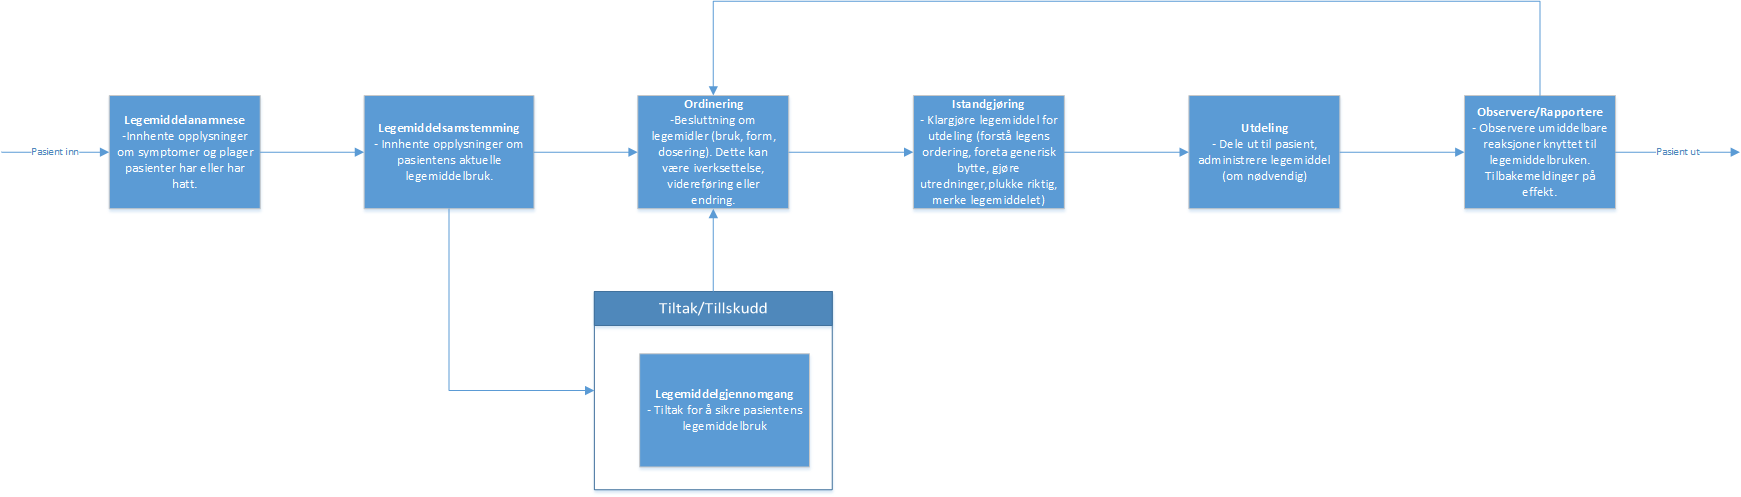
\includegraphics[width=18cm]{images/Legemiddelhandtering}
\label{fig:legemiddelhanderingsprosessen}
\caption{Legemiddelhåndtering i omsorgstjenesten}
\end{figure}
 
\subsection{Legemiddelanamnese} 
Riktig og fullstendig informasjon om pasientens pågående legemiddelbruk i sykehus er viktig for at all videre behandling skal bli så god som mulig. Anamnese er et medisinsutrykk for å hente informasjon som er basert på opplysninger som er gitt av pasienten selv. En anamnese skal inneholde opplysninger som symptomer og plager pasienten har eller har hatt. Anamnesen skal dokumenteres i pasientjournalen. Flere sykehus har et samarbeid i tverrfaglig team for å kunne sikre opptaket av anamnesen.

\subsection{Legemiddelsamstemming}
Da anamnesen skal ha informasjon om symptomer og plager til den enkelte pasient, skal en samstemming ta for seg legemidlene. En samstemming er en metode som helsepersonell, i samarbeid med pasient, utfører for å sikre korrekt overføring av pasientens aktuelle legemiddelbruk. Samstemmingen handler om at sykehuset, fastlegen, hjemmetjenesten, sykehjemmet, pårørenden og pasienten selv skal ha lik informasjon om pasientens faste legemidler. Hensikten er å sørge for at legemiddelinformasjon overføres korrekt ved overganger i pasientforløpet. Ved hver overgang sikres det at tiltak iverksettes for å sikre at det ikke er utilsiktede endringer som ikke indikeres. Dette kan være endringer i form av seponeringer, doseendringer eller ordinasjon. Hvis det er uoverensstemmelser i opplysningene skal dette redgjøres for og dokumenteres i pasientjournalen. 

\gls{lib} er en liste over legemidlene en pasient går på. Dette er en liste som blir laget under legemiddelsamstemming. Når denne listen blir laget skal tilgjengelige kilder brukes. Dette er kilder som EPJ, henvisning, epikrise, e-resept, multidose, PLO-melding eller pasientens egen liste. Her er det også viktig at det blir spurt om legemidler pasienten ikke tåler. \gls{lib} skal inneholde produktnavn, virkestoff, legemiddelform, styrke, dosering og bruksområde.\citep{Legemiddelverket_LMG}
 
\subsection{Ordinering}
Ordinering er prosessen der rekvirent bestemmer bruk av legemidler og at dette journalføres jf legemiddelhåndteringsforskriften §3 bokstav g. En ordinering kan være bestemmelse om å iverksette legemiddelbruk, videreføring, seponering eller endring av dosering. Rekvirent kan være lege, tannlege eller helsesøster. Ordinering skjer på bakgrunn av en faglig vurdering der rekvirent har sett behov for en endring av  pasientens legemiddelbehandling. I denne faglige vurderingen skal rekvirenten påse at bruken av legemidlene er forsvarlig for pasienten, som innebærer interaksjoner med andre legemidler, helsesituasjon, allergier og mer. 

Etter å bestemme bruk av legemidler må de bestilles. Rekvivering er prosessen ved muntlig, skriftlig eller elektronisk bestilling av legemidler jf legemiddelhåndteringsforskriften §3 bokstav f og forskrift om rekvirering og utlevering av legemidler fra apotek §1-3 bokstav e.  

\subsubsection{Legemiddelgjennomgang}
\ot{Forklar kort}
\ot{Tydeliggjør hvor dette skjer, konteksten.}
\ot{Ref forrige kap på en eller annen måte}
Tiltak for å sikre pasientens legemiddelbruk.

 

\subsection{Istandgjøring}
Istandgjøring er prosessen med å klargjøre legemiddel for utdeling jf legemiddelhåndteringsforskriften §3 bokstav i. Istandgjøring skal som hovedregel skje på grunnlag av orderingen gjort til enkeltpasient. Prosedyren er fastsatt av virksomhetsleder og utarbeidet av helsepersonell med rekvireringsrett for pasienten. Helsepersonellet som håndterer legemiddlene må forstå legens ordinering, eventuelt foreta generisk bytte\footnote{Generisk bytte er bytte til et likeverdig legemiddel som inneholder samme virkestoff i samme
mengde og i samme formulering.}, gjøre utredninger, sørge for å plukke riktig legemiddel og merke legemiddelet dersom legemiddelet ikke deles ut direkte. \citep{forskrift_legemiddelhandtering}

\subsection{Utdeling}
\ot{Hvem utdeler og hvor?}
Utdeling er prosessen hvor ferdig istandgjort legemiddel skal leveres ut til pasienten. Den som deler ut legemidlet må også kvalitetsikre utdeling. Dette vil si at den som leverer ut også skal observere inntaket, eventuelle umiddelbare eller senere reaksjoner av inntaket. Det må også vurderes og dokumenteres virkning og eventuell ikke-virkning av inntaket. Utdeling av legemidlene skal dokumenteres.

\subsection{Observere/Rapportere}
For å kunne ha en forsvarlig behandlig av pasienten må det oppstå regelmessige observasjoner av pasient. Med observasjon menes både observasjon av umiddelbare reaksjoner på gitt legemiddel og eventuelle reaksjoner som oppstår senere, men som kan knyttes til legemiddelbruken. Det må også komme tilbakemeldinger på manglenede effekt. Helsepersonell har også ansvar for å rapportere hvis det oppstår mistanke om kvalitetsvikt på legemidler eller utstyr. Observasjoner skal rapporteres til behandleransvarlig og dokumenteres i pasientjournalen.\citep{forskrift_legemiddelhandtering}


\section{Informasjonskilder og retningslinjer} \label{Informasjonskilder_og_retningslinjer}
I dette kapittelet skal vi se på ulike informasjonskilder og retningslinjer klinikere kan bruke når de foretar legemiddelgjennomganger i tillegg til legemiddelinformasjon.
\subsection{Pasientjournal} 
\subsection{Felleskatalogen}
Felleskatalogen er et oppslagsverk over farmasøytiske preparater til salgs i Norge. Her finnes en oversikt over preparater, vaksiner, naturlegemidler samt register over ATC-koder og substanser. I tillegg er det informasjon om spesielle tema som blant annet graviditet og forgiftning. All informasjon i felleskatalogen er enkelt tilgjengelig i et fritekstsøk. Felleskatalogen gis ut årlig og sendes ut gratis til alle helsepersonell-og institusjoner i Norge.
\subsection{RELIS}
Regionale legemiddelinformasjonssentre(RELIS) er en virksomhet som gjennom produktuavhengig legemiddelinformasjon har et mål om å bidra til rasjonell og korrekt legemiddelbruk. RELIS er i fire ulike regioner som holder kurs og seminarer for blant annet allmennleger og kliniske farmasøyter omkring riktig bruk av legemidler. RELIS har en felles nettside (www.relis.no) som publiserer nyheter og problemstillinger ved legemiddelbruk. Nettsiden har også en spørsmål-svar database for legemiddelrelaterte spørsmål. Her kan helsepersonell få hjelp, samtidig som at alle kan se tidligere spørsmål og svar. RELIS gir også muligheten for helsepersonell å melde inn bivirkninger via nettsiden. Avsender får en tilbakemelding etter en vurdering RELIS tar. Disse bivirkningene registreres også i en nasjonal bivirkningsdatabase.
\subsection{Renal Drug Database}
Renal Drug Database er en ressurs sammensatt av flere ulike kilder for å tilby helhetlig legemiddelinformasjon i forbindelse med pasienter som har nedsatt nyrefunksjon. Databasen tilbyr over 800 monografer med informasjon om klinisk bruk, interaksjoner, metabolisme og administrering. Denne ressursen er satt sammen av eksperter på området innenfor nedsatt nyrefunksjon og farmasi i Storbritannia. Med lisens har man full tilgang til kvalitetssikrede monografer, søkefunksjoner og verktøy som blant annet beregner Cockroft-Gault. Kliniske farmasøyter i Midt-Norge har lisens på Renal Drug Database.
\subsection{Epikrise}
Epikrise er en sammenfattet tekst som redegjør for årsak, utvikling og behandling av en pasient etter endt behandling. I de fleste tilfeller sendes epikriser etter endt sykehusopphold. Epikrisen sendes ut i henhold til §9 i pasientjournalforskriften. Pasienten har rett til å opplyse hvem epikrisen skal sendes til, men dersom ikke dette er spesifisert vil mottagere være henvisende helsepersonell samt pasientens fastlege. Motivasjonen bak epikrise er å sende relevant informasjon etter endt behandling til helsepersonell, slik at pasienten får nødvendig og forsvarlig oppfølging.

Det er ingen satte standarder i Norge for epikrisens struktur og innhold, men det finnes flere veiledninger omkring dette. Helsedirektoratet har utgitt en rapport som presenterer forslag til krav for innhold og struktur av den faglige delen av epikriser \citep{Den_gode_epikrise}. I rapporten er disse kravene kategorisert etter om de skal være obligatoriske eller anbefalte krav, i tillegg til når disse skal eller bør innføres. Hvorvidt disse kravene blir aktivt møtt er uvisst. I følge denne rapporten bør epikrisen, i tillegg til å ha praktisk informasjon om sykehus,utskrivende lege, tidspunkt og mer, inneholde informasjon om blant annet årsak til innleggelse,diagnose, kliniske prosedyrer, legemidler ved utskrivning, og vurdering. Siden denne informasjonen er ustrukturert, sendes epikrisen som fritekst.

\subsection{START, STOPP og NorGeP}
Screening Tool to Alert to Right Treatment(START) er en sjekkliste for forskrivning av legemidler til eldre. START er utviklet i Irland men er blitt oversatt til norske forhold. Listen brukes altså ved forskrivningsprosessen, og er delt opp i kapitler inkludert muskel- og skjelett, hormonsystemet, hjerte-og karsystemet, luftveien og mer. Under hvert kapittel er det forslag til legemidler eller type legemiddel som bør forskrives ved bestemte sykdommer.

Screening Tool of Older Persons’ Prescriptions er en sjekkliste for potensielt uhensiktsmessige forskrivninger til eldre. Denne er også utviklet i Irland og oversatt. Listen er strukturert på likt vis, og med mange av de samme inndelinger av kapitler. Her er det også listet legemidler under kapitler som går på ulike kroppsdeler/funksjoner, men her er dette legemidler som er uhensiktsmessig. Både i START og STOPP er det ingen detaljert forklaring på hvorfor typer legemidler bør forskrives eller seponeres.

The Norwegian General Practice(NorGeP) criteria er en liste over 36 kriterier over farmakologisk uhensiktsmessige forskrivninger til eldre pasienter i allmennpraksis. Her er legemidler gruppert etter område og beskrevet med generiske navn, i tillegg til en kort kommentar.

Felles for disse kriteriene er at de skal være til hjelp for å redusere suboptimale forskrivninger for eldre. En irsk studie har vist at bruken av START og STOPP gir resultater i praksis \citep{START_STOPP_GALLAGHER}. I hvor stor grad disse kriteriene er i bruk i Norge er uvisst. Samtidig kan kriteriene ha blitt en del av rutinen, slik at selve sjekklistene ikke blir brukt eksplisitt. START,STOPP og NorGeP er enkelt tilgjengelig for alle, så bruken av disse vil være vanskelig å måle. Flere fagpersonell vi har hatt kontakt med er kjent med disse kriteriene, og har samtidig uttrykt at disse ofte er satt opp på pauserom og lignende arealer, som en huskelapp.  
\subsection{E-resept}
\subsection{Legemidler i bruk}
Legemidler i bruk er meldinger som er en del av e-resept, og inneholder alle legemidler og andre relaterte varer som inngår i en samlet bruk for en pasient. Disse meldingene erstatter bruken av ordinasjonskort som før var i bruk i forbindelse med multidosering. Meldingen sendes fra multidoseringsansvarlig lege til apotek.
\subsection{Legemiddelhåndboka}
Norsk legemiddelhåndbok er et oppslagsverk om legemidler som behandling. Den er beregnet for allmennleger og institusjonslegen der vedkommende ikke er spesialist innenfor området. Derfor er det lagt vekt på å omtale tilstander som behandles hovedsakelig av disse legene, hvor legemidler har en viktig plass i behandlingen. I motsetning til FEST inneholder dette oppslagsverket detaljert informasjon om indikasjoner og bivirkninger av legemidler. Legemiddelhåndboken er delt inn i fire deler: 
\begin{itemize}
  \item Terapikapittler som tar for seg sykdommer i samsvar med WHOs sykdomsklassifikasjon
  \item Legemiddelkapittler som hører inn under terapikapittlene
  \item Generelle kapittler tar for seg grunnkunnskap innenfor farmakologi, og refusjonsreglene
  \item Registre 
\end{itemize}
Norsk legemiddelhåndbok finnes fritt tilgjengelig på nett i flere formater(\url{http://legemiddelhandboka.no/}), og som mobilapplikasjon.
\section{Kodeverk og standarder}
\subsection{ICD}
\gls{icd} er et internasjonalt kodeverk for klassifisering og registrering av sykdommer og andre beslektede helseproblemer. \gls{icd} er vedlikeholdt av \gls{who}, som er en del av FN. Alle sykdommer er klassifiserbare med bruk av \gls{icd}. Kodeverket er delt inn i ulike kapittler som igjen har sine egne kategorier. \gls{icd} blir oppdatert ved behov, og siste versjon er ICD-10 som ble publisert i 1994\citep{WHO_ICD}. Det er opp til hvert enkelt land å bestemme hvilken versjon av \gls{icd} man velger å benytte. I USA bruker de fortsatt ICD-7 fra 1962, men har samtidig oppdatert og tilpasset denne for å møte deres behov. Videre må \gls{icd} tilpasses og oversettes, da flere land har særegne klassifikasjoner.

I Norge brukes ICD-10 som er oversatt av KITH(Helsedirektoratet,avd standardisering). I Norge brukes dette kodeverket blant annet i spesialisthelsetjenesten, men også i andre områder som for eksempel i SSB for koding av dødsårsaker\citep{KITH_ICD}. Primærhelsetjensten bruker kodeverket ICPC.
\subsection{ICPC}
International Classification of Primary Care (ICPC) er et internasjonalt kodeverk for dokumentasjon av helseproblemer, diagnoser og symptomer som er brukt i primærhelsetjenesten. Her blir dette brukt ved konsultasjoner, henvisninger og forskriving av legemidler. Eksempelvis krever NAV at dette kodeverket brukes på alle attester der årsaken er sykdomsrelatert. ICPC ble første gang publisert 1987, og er utviklet av WONCA International Classification Committee(WICC). ICPC er nå i andre versjon og revideres fortløpende. I Norge brukes siste versjon, som er oversatt av KITH. 
\subsection{ATC}
Anatomisk, terapeutisk klassifikasjon(ATC) er et kodeverk som brukes for å inndele legemidler etter hvilket organ det virker på samt legemidlets virkemåte og egenskaper. Klassifiseringen brukes som basis for legemiddelstatistikk, i FEST(2.2.2) og i tilknytning til ICD-10(2.3.1). Systemet utvikles og vedlikeholdes av WHO.
\subsection{SNOMED-CT}
Systemised Nomenclature of Medicine-Clinical Terms (SNOMED-CT) er en terminologi som inneholder medisinske begrep, synonymer, koder, og definisjoner som er brukt i klinisk dokumentasjon. SNOMED-CT er ansett som den mest omfattende og flerspråklige terminologien for klinisk helsevitenskap\citep{Health_interoptability_HL7_SNOMED}. Hovedsakelig brukes denne for å gi bedre kommunikasjon og interoperabilitet på tvers av platformer. Norge er det eneste skandinaviske landet som ikke er medlem av IHTSDO.

\section{Personvern}\label{Personvern}
Digitale løsninger som bruker informasjon og personopplysninger gir store muligheter, men også visse problemstillinger knyttet til personvern. Behandling av sensitive opplysninger digitalt har den fordel med at det er lett tilgjengelig både internt i institusjonen i tillegg til pårørende og pasienten. Samtidig kan denne fordelen føre til at det blir enklere for uvedkommende å få tak i denne informasjonen. Dette kapittelet tar for seg lover og forskrifter som skal ivareta personvernet ved bruk av pasientspesifikk informasjon, og i vårt tilfelle i beslutningsstøttesystem.
\subsection{Personopplysningsloven og helseregisterloven}
Både personopplysningsloven og helseregisterloven har krav til informasjonssikkerhet. Det er Datatilsynet og Helsetilsynets ansvar for å se til at regelverket blir fulgt. Helseregisterlovens formål er "å legge til rette for innsamling og annen behandling av helseopplysninger (...) og gi bedre helse-og omsorgstjenester", jf. §1. Pasientspesifikk informasjon brukt i et beslutningsstøttesystem går i helseregisterloven under definisjonen av helseopplysninger jf. §2 punkt a. 

Personopplysningsloven er ment til å bidra til at personopplysninger skal behandles i tråd med grunnleggende personvernhensyn og informasjonssikkerhet. Helseregisterloven har regler for hvordan innsamling og behandling av helseopplysninger skal foregå. Reglene i helseregisterloven går i tråd med kravene som angår behandling av personopplysninger i personopplysningsloven. Begge lovene tar utgangspunkt i EUs personverndirektiv (95/46/EF).          

\subsection{Medisinsk utstyr}
Lov om medisinsk utstyr skal regulere "produksjon, markedsføring, omsetning og bruk av medisinsk utstyr", jf. §1. Dets formål er å "forhindre skadevirkninger, uhell og ulykker, samt sikre at medisinsk utstyr utprøves og anvendes på en faglig og etisk forsvarlig måte", jf. lovens §2. Loven gir klare detaljer om krav, merking og markedsføring, lagring og veiledning ved salg samt informasjon og bruk av medisinsk utstyr.

Lovens definisjon av medisinsk utstår er "(...)ethvert instrument, apparat, hjelpemiddel, materiale eller enhver annen gjenstand (...) ment å skulle brukes på mennesker", jf. §3 første ledd. Her er det en usikkerhet hvorvidt beslutningsstøtte med bruk av pasientspesifikk informasjon går under denne definisjonen. Lov om medisinsk utstyr §3 fjerde ledd, sier at i tvisttilfeller er det opp til Helse-og omsorgsdepartementet å avgjøre om et produkt faller innenfor kategorien av medisinsk utstyr.   

\subsection{Normen}
I 2002 tok Helsedirektoratet initiativ til å utvikle et sett med regler for trygg og sikker informasjonsutveksling. Dette initiativet kalles Normen, som utarbeider retningslinjer og krav for informasjonssikkerhet mellom ulike parter i helsesektoren. Normen er utviklet av representanter fra flere felt innenfor helse-, omsorgs- og sosialsektoren. Virksomheter kan forplikte seg ved avtale å følge Normen\citep{Normen}.

\section{Beslutningsstøtte}
\subsection{Klinisk beslutningsstøtte}
Klinisk beslutningsstøtte finnes i flere former som for eksemel retningslinjer som START og STOPP kriterier \citep{Bedre_legemiddelbehandling_av_eldre}. Evidensbasert medisin danner grunnlaget for slike retningslinjer ved bruk av randomiserte kliniske forsøk \citep{what_is_ebm}. Innen klinisk beslutningsstøtte har vi ikke kun slike "analoge" løsninger, men også digitale beslutningssystemer. Disse systemene kombinerer medisinsk kunnskapsdatabaser og algoritmer med spesifikk pasientdata og skal gi klinikere/brukere forslag til diagnose, prognose, monitorering eller behandling av individuelle pasienter \citep{european_commission}. 


\subsubsection{Evidensbasert medisin}
Innen forskning er en nødt til å ta hensyn til bevis. Medisin har i løpet av de siste 100 årene beveget seg gjennom faser hvor vi har gått fra at leger gjør seg opp egne meninger på hva som fungerer. Til enkle observasjoner innen medisin hvor pasienten av en eller annen grunn ikke ville motta behandling. Problemet med slike observasjoner er at de gruppene som mottar behandling og de som ikke gjør det ikke er tilfeldig valgte personer. Hvis en ser på litteraturen kan det se ut som sammenligningsgruppene se ut som en god miks fra populasjonen, men i virkeligheten kan det være andre grunner til at kontrollgruppen ikke fikk behandling. Hvis de i kontrollgruppen selv har valgt at de ikke vil ha behandling kan det være på grunn av for eksempel, en alternativ levestil. Dette kan resultere i at de på andre måter påvirker resultatet av studien på andre måter \citep[s.20-21]{cochrane1972}. Når en skal vurdere kriteriene for suksess kan en for eksempel vurdere subjektive kriterier som grad av effekt, men det enkleste er å ta hensyn om pasienten er død eller levende en viss periode etter behandling.

Det finnes bedre måter å utføre slike eksperimenter på, vi kan minimere slike mindre tilfeldige inndelinger av forsøksgruppen ved bruk av randomiserte, kontrollerte studier. I stedet for å se på "naturlige" inndelinger av forsøkspersonene skal gruppene bli valgt tilfeldig. Hverken pasient eller lege burde vite om pasienten er i kontrollgruppen eller ikke. Når legen heller ikke vet gruppen til pasienten blir dette kalt en "double blind" \citep[s.22-s23]{cochrane1972}. For å gjøre forsøkene så troverdige som mulig kontrolleres forsøkgruppen nøye slik at de passer inn under de kriteriene som legges til grunn. For eksempel kriterier som alder, diagnose og kjønn, dette for å prøve å luke ut ytre påvirkninger. Resultatet av slik forskning er veldig spesifikke resultater som passer til spissede forsøksgruppen.


\subsubsection{Kliniske retningslinjer}
Kliniske retningslinjer har sitt evidensgrunnlag fra evidensbasert medisin. Resultatet av slik forskning kan gi anbefalinger til behandling for veldig spesifikke tilfeller. Problemet med slike anbefalinger er at det nødvendigvis ikke passer veldig bra med populasjonen for øvrig.

Et stort problem, og økende  er problematikken rundt multimorbide. Multimorbide, pasienter med $\geq$2 kroniske lidelser, står for ca. 27\% av populasjonen og 66\% av de totale utgiften til helsevesenet i USA \citep{managing_MCC}.  Etterhvert som populasjonen øker, vil dette bli et enda større problem. I 1950 var det 8\% av populasjonen som var eldre enn 67 år, i dag er tallet 14\% og i 2050 er det estimert med 21\% eldre \citep{SSB_dette_er_norge}. Dette er en betydelig økning i eldre, og sammen med at over 50\% av populasjonen over 65 år er multimorbide, blir dette problem for fremtiden \citep[s.178]{OECD_health_reform}.



\subsubsection{Ekspertsystemer}


Ekspertsystemer er en gren innen kunstig intelligens(KI).\ot{nei, kunnskapsteknologi- som gir en beng i menneskelig resonnering eller kunnskap. Derimot korrekt og forutsigbar resonnering.} Dette er systemer som skal ha kunnskap om det domenet de er designet for og skal ha mulighet til å løse problemer innen dette domenet. Typiske bruksområdet ligger innenfor datatolkning(sonarsignaler) og diagnostisering av feil(feil i utstyr eller sykdom i mennesker), samt analyse av kompliserte strukturer og planlegging av avgjørelser for en robot \citep[s.2]{intro_expertsystems}.

Det som skiller et ekspertsystem fra et vanlig dataprogram er:
\begin{itemize}
\item Simulere menneskelig resonnement innen problemdomenet i stedet for å simulere domenet i sin helhet.
\item Skal utføre resonnement over en representasjon av menneskelig kunnskap. Kunnskapen til systemet er ofte skrevet i et språk designet for kunnskaprepresentasjon. Kunnskapen er moddelert i en kunnskapsbase og systemet resonnerer med en "inference engine" samt annen logikk.
\end{itemize}\citep[s.3]{intro_expertsystems} 


Ekspertsystemer er systemer som løser problemer med realistisk kompleksitet som ofte krever menneskelig tolkning. De skal løse virkelige problemer innen forskning eller av kommersiell interesse. Systemet må ha en høy ytelse, både i hastighet og robusthet. Et slikt system opererer som en ekspert og brukeren av systemet forventer svar innen rimelig tid. Systemet skal også kunne gi en forklaring for sitt resonnement og løsning, slik at brukeren kan se grunnlaget for beslutningen\citep[s.3]{intro_expertsystems}.

Kunnskapsbasen fylles med ved et samarbeid mellom en informatiker og en ekspert innen domenet systemet skal lages for, for eksempel en lege. Innhenting blir ofte en flaskehals under utvikling av slike systemer og det er estimert at et slikt team kan lage mellom 2 og 5 fakta om dagen. Problemer innebærer forskjellig fagspråk, en ekspert har ofte problemer med å formidle sin kunnskap i et dagligdags språk. Eksperter trenger også å vite mer enn bare de enkle fakta og prinsipper om et domene for å løse problemer. For eksempel, de vet hvilken informasjon som er relevant for det problemet de skal løse. De er også flinkere på å dele vanskelige problemer ned i mindre, enklere problemer som kan løses individuelt. Å modellere slik kunnskap, som ofte er basert på personlige erfaringer er mye vanskeligere og kan være en svakhet til et slikt system\citep[s.3-4]{intro_expertsystems}.

\subsection{Juridiske problemer knyttet til beslutningsstøtte}
Beslutningsstøtte skal hjelpe en bruker med å fatte en korrekt beslutning, men hvilken part er skyldig hvis en beslutning fattet ved hjelp av beslutningsstøtte, får kritiske konsekvenser?  Dette er en problemstilling som berører både brukeren, beslutningsstøttesystemet i tillegg til eventuelle forfattere av innholdet brukt i systemet. Er for eksempel en juridisk ansvarsfraskrivelse tilstrekkelig for å unngå et søksmål? Hvis informasjonen og reglene brukt i beslutningsstøttesystemet er åpne og fritt tilgjengelige data, kan forfatterne bak innholdet da være skyldige?

Her er det dessverre ikke noen definitive svar. En artikkel fra 2007 som så på muligheter og problemstillinger knyttet til bruk av SOA(Service-Oriented Architecture) i kliniske informasjonssystemer,  
sier at tjenester er ikke lisensierte klinikere, så juridisk vil institusjonen eller utøveren være ansvarlig for å se bort i fra råd gitt av systemet som kan være skadelige\citep{SOA_DSS}. Videre argumenterer forfatterne at dette utgangspunktet kan minske brukernes tillit til bruken av disse tjenestene. Her må vi si oss uenige, da dette også kan sies om anvendelsen av retningslinjer, kildereferanser og annen litteratur innenfor medisin. Disse er mye brukt, selv om forfatterne ikke tar ansvar for eventuelle konsekvenser.

\section{Teknologi\ot{Veldig langt kapittel(mangler mye subsections), kan vi flytte ut til eget kapittel? Veldig sentralt for oss dette}}
I dette kapitellet ser vi på teknologi som eksisterer og som i tillegg kan være til nytte i å svare på forskningspørsmålet jf. delkapittel \ref{innled:forskningsporsmal}. 
\subsection{Ontologi}
\label{bakg:ontologi}
I kunnskapsteknologisk litteratur finnes det flere definisjoner om hva en ontologi er, og mange av disse er i strid med hverandre. For formålet med vårt studie er en ontologi et konsept som presist formulerer beskrivelser i et domenet. I en ontologi inneholder det klasser (også kalt konsepter), egenskaper som beskriver funksjoner og attributter for hvert konsept og restriksjoner for egenskapene. En ontologi sammen med et sett av instanser utgjør en kunnskapsbase. Et instans er et objekt av en klasse.\\
Klasser er sentralt i ontologier. Klasser beskriver konsepter i et domene, for eksempel kan vi ta for oss klassekonseptet mennesket. Et hver spesifikk menneske vil da være et instans av klassen Mennesket. Håvard Moås ville vært et naturlig instans av klassen Mennesket. Klasser kan også ha subklasser, hvor en artist kunne vært en subklasse av klassen person. \\
Egenskaper (properties) beskriver egenskaper til en klasse og ett instans. Håvard Moås har egenskaper ved å være et menneske, mennesker har et kjønn og finnes i forskjellige raser. Her har vi da to egenskaper som kobler mennesket sammen med et kjønn og rase. (Visualisert i figur 4.1). Under hver klasse er det instanser av hver klasse. For å ha resonneringstøtte kan inverse og symmetriske egenskaper være lurt, vi vil komme nærmere tilbake til dette i kap 4.2.4. % TODO: se over at kapittel stemmer


\begin{figure}[H]
\centering
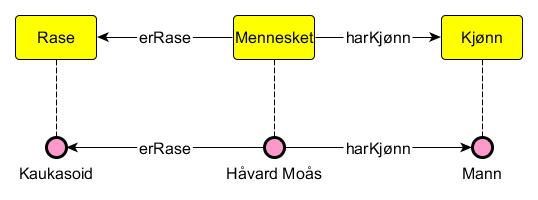
\includegraphics[width=10cm]{images/ontologi_eksempel.jpg}
\caption{Eksempel på klasser og egenskaper i en ontologi }
\end{figure}

I praksis inkluderer utvikling av en ontologi å:
\begin{itemize}
\item Definere klasser i ontologien.
\item Arrangere klassene i et taksonomisk (subklasser-subegenskaper) hierarki.
\item Definere egenskaper og beskriv lovlige verdier for disse egenskapene.
\item Fylle inn verdier for disse egenskapene og klassene i form av instanser.
\end{itemize} \citep{ontology_101}
\subsection{Semantisk teknologi}
\subsubsection{Visjon}
Det er ingen fast definisjon på semantisk web, men heller en visjon om at maskiner skal kunne forstå meningen bak innholdet på internett. Begrepet er skapt av W3C, som også  utvikler, vedlikeholder og tilrettelegger teknologier og metoder som brukes for å realisere denne visjonen. Ifølge skaperne av begrepet “gir semantisk web et felles rammeverk som tillater data til å bli delt og gjenbrukt på tvers av applikasjoner, bedrifter og samfunnets grenser”\citep{W3C_semantic_web}.  

For å realisere denne visjonen må det tas designvalg for semantisk web. Disse kan bli summert slik: 
\begin{enumerate}
    \item lage strukturerte, semi-strukturerte data tilgjengelig i standardisert format på web;
    \item ikke bare lage datasett, men også individuelle dataelementer og deres relasjoner 	tilgjengelig på web;
    \item Beskrive den tiltenkte semantikken i en formalisme, slik at den tiltenkte semantikken kan prossesseres av maskiner\citep{webprimer}.
\end{enumerate}
Det er mange muligheter som oppstår ved å gjøre webens innhold mer tilgjengelig for maskiner. Maskiners rolle i den tradisjonelle weben er for det meste å overføre informasjon fra tjener til klient og indeksere søkeord. Ved hjelp av semantisk web kan maskiner gjøre mye av det intelligente arbeidet, som for eksempel aggregering og kombinering av data. Søking trenger ikke å være begrenset til nøkkelord; Ved hjelp av semantisk forståelse av selve søket kan dette inkludere synonymer, hensikt, kontekst av søk med mer. Nettsider kan bli mer personlig tilpasset hvis spesifikke agenter kan forstå innholdet av nettsiden og samtidig tilpasse dette til brukerprofiler.    
\subsubsection{Semantiske teknologier}
De designvalg som er nevnt tidligere må også være beskrevet i bestemte teknologier. Disse teknologiene er også basisen for semantisk web, som beskrevet av W3C:
\begin{enumerate}
\item Grafer som datamodell for objekter og deres relasjoner, der et objekt er en node i grafen og en kant representerer relasjoner mellom objekter. For dette brukes RDF(Resource Description Framework).
\item Web-identifikatorer(URI) for å identifisere objekter og relasjoner. Disse er også beskrevet i RDF.
\item Ontologier som datamodell for å representere den tiltenkte semantikken av data. Her brukes OWL(The Web Ontology Language) og RDF Schema som formalismer, som igjen bruker URI for å representerer typer og egenskaper.
\end{enumerate}

Videre må det også være mulig å hente og manipulere data fra disse strukturene gjennom spørringer. SPARQL er et spørrespråk utviklet av W3C som også har gjort dette til en standard.  

Semantisk web kan tenkes å være utviklet lagvis, der hvert lag er bygget oppå et annet lag. Grunnen til denne lagdelingen er todelt. En ting er at det er enklere å få konsensus i miljøet for små steg som tas enn større endringer foreslås. Fra et annet perspektiv er denne lagdelingen viktig med tanke på standardisering. I utviklingen av semantisk web er det stor konsensus på at følgende to prinsipper burde bli fulgt når et lag bygges oppå et annet:
\begin{itemize}
\item En programvarekomponent som er oppmerksom på et lag burde være i stand til å forstå og bruke informasjon lagd på lavere nivå. Hvert lag burde altså være nedover kompatibel.
\item Det skal være mulig for en programvarekomponent å delvis ta utnytte av informasjon fra høyere lag. Dette er mulig hvis en kan ignorere komponentene som overgår nettopp laget denne programvarekomponenten er brukt til. Eksempel kan være at en komponent oppmerksom på RDF og RDFS kan delvis tolke informasjon skrevet i OWL. 
\end{itemize}

Denne lagdelte arkitekturen har vært en gjeldende visjon i utviklingen av semantisk web. Dessverre har ikke utviklingen gått helt denne veien, og noen kompromisser har vært nødvendig å ta på bekostning av prinsippet om nedover kompatibilitet. Mer om dette i kap 4.1.3.  % TODO: se over at kapittel stemmer

Figur 4.1 viser den lagdelte arkitekturen for semantisk web. Unicode og URI-laget sørger for at vi bruker internasjonale tegnsett og muliggjør identifisering av objekter. XML-laget med NameSpace og skjemadefinisjon gjør det mulig å integrere definisjoner fra semantisk web med XML-baserte standarder. Med RDF og rdfschema kan man opprette påstander om objekter med URI, samt definere egne modeller. Ontologier er en form for kunnskapspresentasjon. Dette laget sørger for muligheten til å representere mere komplekse relasjoner mellom objekter. Logic-laget kan tenkes å være en utvidelse av Ontologi-laget; Et resonneringssystem for økt funksjonalitet og muligheten til å manipulere applikasjonsspesifikk deklarativ kunnskap. Trust-laget sørger for utførelsen av reglene definert av ressonneringssystemet, og sammen med Proof-laget utgjør mekanismen for applikasjoner å stole på bevis. De to øverste lagene i modellen skal sikre kvaliteten på informasjonen.

\begin{figure}[H]
\centering
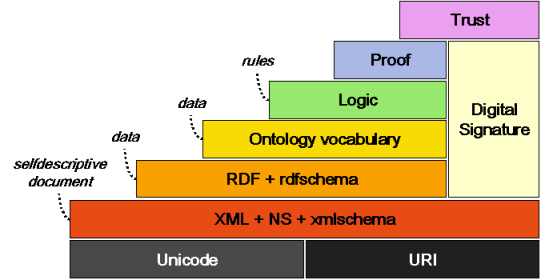
\includegraphics[width=90mm]{images/swlevels.png}
\caption{Semantisk web lag }
%\label{overflow}
\end{figure}

\subsubsection{Open world assumption}
Open world assumption er et prinsipp brukt i forbindelse med kunnskapsrepresentasjon, som sier at et utsagn kan være riktig uavhengig av om man \textit{vet} at utsagnet er riktig eller ikke. Dette er da det motsatte av det som kalles "Closed-world assumption", som sier at ethvert utsagn som er riktig faktisk er riktig. Semantisk web kan ikke ha et "closed-world assumption", siden en kan aldri vite om flere ressurser er beskrevet på flere ulike måter ute på internett. I tillegg kan man ikke vite om disse er beskrevet med bruk av samme type skjema eller ha like egenskaper. Et eksempel på dette kan være at man har flere universiteter, og noen av disse er mer beskrevet enn andre, og kanskje bruker et annet vokabular i tillegg. Instansene kan også beskrive samme universitet! 

\subsubsection{Resource Description Framework}
RDF er et formelt språk brukt for å beskrive informasjon. I motsetning til HTML og XML, der målet er å vise dokumenter riktig, er målet til RDF å bevare meningen bak dokumentet på tvers av applikasjoner på web. På denne måten kan denne informasjonen prosesseres videre og kombineres på ulike måter. RDF er ansett som det grunnleggende representasjonsformatet ved utviklingen av Semantic Web.

Kort sagt beskriver RDF generelle relasjoner mellom ressurser. RDF er basert på en graf-orientert dataskjema, der et dokument beskriver en rettet graf. Med andre ord har man et sett med noder som er lenket med direkte kanter. Både nodene og kantene er merket med unike ID'er. En node kan unntaksvis være blank, altså at den representerer objekter som ikke har egne navn. En ID kan være i form av et navn eller en Uniform Resource Identifier. Sistnevnte er en generalisering av URL(Uniform Resource Locator), som er en streng brukt til å finne websider i en nettleser. Med andre ord så er URI en identifiserbar og navngitt ressurs ved hjelp av lokaliseringsinformasjon.

Nodene og kantene i RDF-dokumenter blir omtalt som tripler. Dette er en setning med strukturen subjekt-predikat-objekt. En slik trippel danner en rettet graf, der kantene er forbindelsen mellom to ressurser. Med andre ord representerer kantene i en RDF-trippel forholdet mellom to ressurser. På denne måten kan RDF gi muligheten til å dele strukturert informasjon på tvers av applikasjoner.

\begin{figure}[H]
\centering
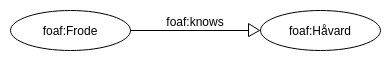
\includegraphics[width=90mm]{images/rdf_triple.png}
\caption{Eksempel på RDF trippel}
% \label{overflow}
\end{figure}
\subsubsection{Resource Description Framework Schema}
RDFS er et sett med klasser og tilhørende egenskaper bygd på RDF; Et vokabular for RDF som gir ytterligere ekspressivitet. Disse klassene og egenskapene gjør at RDFS kan sees på som et språk for kunnskapsrepresentasjon eller et ontologispråk, som kan i stor grad beskriver semantisk gjensidige avhengigheter innenfor et domene. Selv om RDFS kan sees på som et ontologispråk, har den sine begrensninger. Derfor er det mange som kaller RDFS et representasjonsspråk for lettvekts-ontologier. Mer sofistikerte applikasjoner krever et mer ekspressivt representasjonsspråk. Andre vokabularer av RDF, for eksempel OWL, bruker RDFS i bunn. 

Klasser og egenskaper i RDFS kan på flere måter sees likt på som i objektorienterte programmeringsspråk. En kan for eksempel tilegne en instans av en klasse egenskaper til en annen klasse. En hund har den egenskap at den er et dyr. Likevel er det fundamentale forskjeller. Alt i RDFS er klasser, også egenskaper. Egenskaper i RDFS er igjen instanser av klassen rdf:property, som igjen er en instans av klassen rdf:class. Klassehierarkier i objektorientert programmering representerer strukturer som kan sees på som mer statisk. Ved ontologispråk som RDFS representerer disse hierarkiene informasjon ute på internett som kan være i konstant utvikling. I tillegg til dette er ontologier langt mer fleksible, i og med at denne informasjonen kommer fra heterogene kilder.

RDFS gir mulighet til å beskrive hierarkier av klasser og egenskaper, sette restriksjoner på ressurser, definere ressurser som datatype,literal og ressurs samt definere lister.
\subsubsection{Web Ontology Language}
Web Ontology Language(OWL) er et språk for kunnskapsrepresentasjon i likhet med RDFS; et vokabular for RDF. Som allerede nevnt er RDFS noe begrenset, og tilbyr mer eller mindre kun klasse- og egenskaphierarkier, samt sette flere typer restriksjoner på disse. Ved flere tilfeller så trenger man et mer ekspressivt språk for kunnskapsrepresentasjon. Et eksempel kan være at alle personer har en bursdagsdato, og at ingen person er både mann og kvinne. OWL tilbyr nettopp slik funksjonalitet. 

OWL er bygd på en familie av logikkspråk, eller rettere sagt Description Logics som er laget spesielt for å representere terminologisk kunnskap. Description Logic er en samling språk for kunnskapsrepresentasjon, som inkluderer blant annet OWL. Disse språkene gir mulighet for å beskrive blant annet klassemedlemskap, klassifisering, ekvivalens og likhet, disjunkthet og ulikhet, kardinalitet, sette lokalt "scope". I tillegg til dette tilbyr OWL automatisert resonnementstøtte. Dette sikrer at et ontologi er logisk korrekt, og innebærer sjekk for konsistens og utilsiktet relasjoner mellom klasser og instanser. 

Det er ikke mulig å ha automatisk resonnementstøtte i kombinasjon med ekspressiviteten beskrevet ovenfor. Derfor er OWL delt opp i to ulike subspråk for å fylle de ulike kriteriene.
\subsubsection{OWL Full}
OWL Full er språket i all sin helhet. Det tillater all mulig kombinering av OWL-primitiver med RDF og RDFS. OWL Full har en RDF-basert semantikk som gjør at den er nedover kompatibel. Det vil si at ethvert korrekt RDF dokument er også et OWL Full dokument, og enhver slutning i RDFS er også en korrekt slutning i OWL Full. På en annen side gjør dette, i tillegg til vilkårlig bruk av primitiver, at automatisk resonnementstøtte i OWL Full ikke er mulig. Språket er med andre ord så fleksibelt at det ikke er mulig å trekke noen slutninger om korrekthet.
\subsubsection{OWL DL}
OWL DL er et subspråk av OWL som er "mappet" mot Description Logic. På dette viset er det mulig med god resonnementstøtte. Det eksisterer flere tolkere til dette, inkludert Pellet, FaCT,RACER og HermiT. En bakside ved dette er at det begrenser ekspressiviteten som OWL Full har. 

Den største ulempen ved OWL DL er at den ikke er fullt kompatibel med RDF. Dermed bryter dette med den lagdelte arkitekturen og prinsippet med at hvert lag skal være nedover kompatibelt som beskrevet i kap 4.1. Det er kun ved OWL Full at dette prinsippet blir fulgt, dog på bekostning av muligheten for resonneringsstøtte.    

\subsubsection{SPARQL Protocol and RDF Query Language}
SPARQL er et spørrespråk for å hente og manipulere kunnskap uttrykt i RDF. Spørrespråket er utviklet primært for RDF og har flere likheter med spørrespråk for tradisjonelle databaser. Det finnes flere spørrespråk for RDF, inkludert DQL og N3QL. SPARQL er spørrespråket W3C anbefaler og er gjort til en standard. Fleste populære programmeringsspråk har API'er tilgjengelig for å prosessere og lage SPARQL-spørringer.

For å kunne utføre en spørring må man ha en triple store tilgjengelig, som kan sees på som en RDF-database. I dokumentasjonen for SPARQL refereres disse som "graph store". Hele denne databasen er med andre ord et sett med tripler som beskrevet i kapittel 4.1.2. SPARQL har mekanismer for hente, legge inn og fjerne tripler i en triple store. Man har fire ulike type spørringer i SPARQL, men alle følger et bestemt mønster. Grunnlaget er at en SPARQL-spørring konstrueres som et grafmønster, der databasen finner tripler som har et likt mønster. I SPARQL kan man erstatte subjekt, predikat og objekt med variabel. Hvis en ønsker å hente ut alle tripler fra databasen, er det bare å sende inn et grafmønster med kun variabler. Resultatene av en spørring kan gjøres tilgjengelig på flere maskinlesbare formater, inkludert XML og JSON.

\begin{figure}[H]
\centering
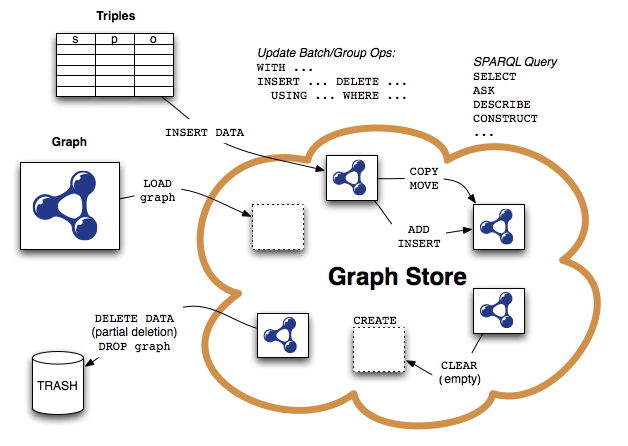
\includegraphics[width=140mm]{images/sparql_endpoint.png}
\caption{SPARQL endpoint }
%\label{overflow}
\end{figure}
%TODO: REFERER DETTE BILDET TIL :https://www.dajobe.org/blog/

\subsubsection{Semantiske teknologier i helse-og biovitenskap}
Mange har sett nytten i å bruke semantiske teknologier innenfor helse-og biovitenskap. Dette feltet har store problemer med heterogene data spredt over ulike domener. Samtidig vokser datamengden i dette feltet. Forskere og andre må kunne foreta spørringer som går på tvers av disse for å kunne ta kritiske avgjørelser. Bruk av semantiske teknologier kan redusere kostnadene ved en slik integrasjon av datakilder. Hvis dette skal være mulig må data om legemidler, sykdommer, pasienter, proteiner, celler og reaksjonsveier være tett integrerte. Samtidig må et felles vokabular må være på plass, med definisjoner, koder, synonymer og begreper. For at sektoren skal kunne se hvilke fordeler bruk av semantisk web innebærer, må en aktør aktivt fremme interesse og muligheter dette fører med seg. W3C opprettet Semantic Web for Health Care and Life Sciences Interest Group for å utvikle, støtte samt være en pådriver for bruken av semantiske teknologier i helse-og biovitenskap\citep{W3C_HCLSIG}. Noe av arbeidet de har gjort er å publisere genomiske og legemiddelrelaterte datasett som RDF-tripler. 

\subsubsection{SNOMED-CT}
For at man skal kunne integrere heterogene datakilder, må et felles vokabular på plass. Systemised Nomenclature of Medicine-Clinical Terms (SNOMED-CT) er en terminologi som inneholder medisinske begrep, synonymer, koder, og definisjoner som er brukt i klinisk dokumentasjon. SNOMED-CT er ansett som den mest omfattende og flerspråklige terminologien for klinisk helsevitenskap\citep{Health_interoptability_HL7_SNOMED}. Hovedsakelig brukes denne for å gi bedre kommunikasjon og interoperabilitet på tvers av platformer. SNOMED-CT er ikke direkte tilgjengelig i OWL-format, men er utgitt som en egen filstruktur kalt Release Format 2. Andre leverandører som Snow Owl IDE\citep{Snow_owl} og skript i ulike programmeringsspråk støtter eksportering til OWL. 

Terminologien eies og drives av International Health Terminology Standards Development Organisation, som ble startet i 2009 av 9 medlemsland. I dag har organisasjonen over 20 medlemsland over hele verden, samtidig som de har gitt ut lisenser for mer enn 5000 individer og organisasjoner\citep{IHTSDO_members}. For å kunne bruke SNOMED-CT eller utvikle programvare som bruker SNOMED-CT må en ha lisens. Norge er det eneste skandinaviske landet som ikke er medlem av IHTSDO. En rapport fra KITH(nå underlagt Helsedirektoratet) fra 2009 konkluderer at SNOMED-CT bør prøves i bruk innenfor et område i helsesektoren der det er et sterkt behov for en standardisert terminologi \citep{KITH_SNOMED-CT}. Samtidig nevnes det at behovene for en slik terminologi vil bli mer åpenbar med tiden, da innholdet i elektroniske informasjonssystemer blir mer strukturert i helsesektoren. Selv om Norge ikke er et medlemsland, er det flere og flere aktører som åpner opp for bruken av denne terminologien. Dips Arena er Dips sitt tredjegenerasjons pasientjournal som kommer til å bruke OpenEHR, som er en åpen kodeplattform for elektronisk pasientjournal. Dette, sammen med arketyper, skal danne basisen for en mer strukturert pasientjournal\citep{Dips_OpenEHR}. OpenEHR har støtte for flere fagterminologier, inkludert SNOMED-CT. I tillegg er det flere arketyper som forutsetter bruk av slike terminologier. Dips Arena er forventet å være ute i produksjon i løpet av 2016. Et nytt norsk insentiv har utviklet en plattform(http://www.magicapp.org/) for å utvikle og oppdatere pålitelige retningslinjer som beslutningsstøtte i elektroniske pasientjournaler(Her menes EMR, hva er det på norsk?). Rammeverket bruker nettopp SNOMED-CT, og andre kjente ontologier i norsk helsevesen som ICD-10, for å komme med pasient-spesifikke anbefalninger\citep{MAGIC_HelsIT}. Selv om flere åpner opp for bruken av SNOMED-CT i Norge, har det aldri vært i klinisk bruk her.

Selv om tanken bak et felles begrepsapparat på tvers av landegrenser virker lovende, har flere institusjoner og land vært avventende til SNOMED-CT. Flere mener at SNOMED-CT i dagens tilstand er utdatert og i overkant komplisert. Samtidig er det også funnet flere kritiske feil i terminologien. En studie \citep{Rector-SNOMED-CT-1} foretok bruk av terminologien i to praktiske prosjekter, for å finne mulige problemstillinger knyttet opp mot denne terminologien og hvordan eventuelt adressere disse. De fant systematiske feil knyttet opp mot sentrale konsepter innen medisin, inkludert hypertensjon og diabetes. Studien konkluderte med at de som brukte SNOMED-CT på denne tiden(2011) burde være varsomme, da feil i hierarkiene eller et forsøk på å rette disse opp ville sannsynligvis føre til meningsløs bruk av terminologien. En nyere studie \citep{Rector-SNOMED-CT-2} studerte SNOMED-CT som et eksempel på å bruke et metodeverk for å finne feil i biomedisinske ontologier, fant ytterligere feil i terminologien som ikke er tidligere oppdaget.

\subsubsection{ICD\ot{vurder å fjern dette? vi nevner det i et tidligere kapittel}}
En annen internasjonal standard for felles terminologi i helseverden er \gls{icd}. Kodeverket er et redskap for klassifisering og registrering av sykdommer og andre beslektede helseproblemer. \gls{icd} er vedlikeholdt av \gls{who}, som igjen er en del av FN.  
\subsection{Informasjonskilder}
\subsubsection{DrOn}
\gls{dron} er en modulær ontologi for legemiddel-produkter utviklet med semantiske teknologier. Den innehar informasjon om ingredienser og biologisk aktivitet med utgangspunkt i legemidler som selges i USA \citep{dron_2013}. Ontologien bruker RxNorm som dets eksterne hovedkilde, som er en medisinsk terminologi som inneholder alle legemidler til salgs i USA. Disse legemidlene er kartlagt opp mot ChEBI-klasser. \gls{chebi} er en database og ontologi som inneholder molekylære entiteter. Resultat av dette er at en kan resonnere mellom legemidler med tilhørende ingredienser og biologiske aktivitet. 

For å lage denne ontologien minet de data fra utgivelser av RxNorm. Dette ble gjort ved å laste ned råfilene, omforme dataene for å deretter importere dette i en relasjonsdatabase ved hjelp av et skript som er tilgjengelig. Så ble RxNorm-entiteter kartlagt opp mot ChEBI-klasser ved hjelp av en konsollapplikasjon som sammenlignet etiketter av ingredienser i RxNorm med klasseannoteringer i \gls{chebi}. Deretter ble den normaliserte databasen oversatt til en OWL-artefakt. 

\gls{dron} er modulært, slik at klasser fra hver kilde er serialisert i separate moduler som igjen er konsumert(del av..) av klasser som er manuelt utarbeidet på et høyere nivå i en modul med termer som «klinisk rolle», «tablett», «kapsel» med mer. På denne måten kan en enkelt bruke deler av ontologien i tillegg til at videreutvikling vil være enklere. 

Denne ontologien inneholder mye informasjon om legemidler, og kan spille en viktig rolle i utviklingen av vårt system. Framgangsmåten deres kan være nyttig for oss, selv om vi velger å ikke ta i bruk \gls{dron}. Hvis vi går for å bruke \gls{dron} på en eller annen måte, er det visse aspekter med ontologien vi må ta stilling til. Den største problemstillingen vil nok være å bruke denne ontologien i norsk sammenheng. Er det mulig å koble amerikanske legemidler opp mot legemidler til salgs i Norge? 
\subsubsection{FEST} \label{FEST}
Forskrivning-og ekspedisjonsstøtte (FEST) er en database utviklet av Statens Legemiddelverk som inneholder oppdatert informasjon om alle legemidler en kan få på resept i Norge. I FEST er det for hvert legemiddel oppgitt informasjon om blant annet pakningsvedlegg, dosering, inntaksmåte, virkestoff og interaksjoner med andre legemidler. FEST brukes som datagrunnlag i systemer for blant annet e-resept, felleskatalogen, interaksjoner.no, allmennlegesystem, kommunal pleie og flere sykehus.

Databasen er i dag tilgjengelig i XML-format. Statens Legemiddelverk jobber nå for å gå bort i fra XML-formatet, og levere FEST som åpne, lenkede data. Dette kaller de femstjerners FEST, som referer til Tim Berners Lee 5-stjerners skala for publisering \citep{Femstjerner_FEST}. Dette innebærer å bruke semantiske teknologier for å gjøre data tilgjengelig på web, samt lage lenker som gir muligheten til å utforske data. En testutgave av femstjerners FEST er tilgjengelig og inneholder kun "varsel fra SLV". Varsel fra SLV(Statens Legemiddelverk) er notis sendt til lege med sikkerhetsinformasjon knyttet til legemidler. Dette kan for eksempel være et varsel om en uheldig bivirkning som ikke er tidligere kjent. 
\subsection{MedExt - Samstemmingsmodul}
MedExt er navnet på samstemmingsverktøyet utviklet av Vivit ved NTNU. Dette verktøyet ble utviklet ved oppdrag fra Norsk forening for allmennmedisin, og brukes i dag av allmennleger i store deler av landet. Medext er en programvarekomponent som er integrert i deres EPJ-system. Her fungerer Medext som prosesstøtte ved samstemmingen av legemiddellister. Det vil si at komponenten vil gjøre det enklere å foreta en samstemming ved å strukturere informasjon fra fritekst og sette denne listen opp mot \gls{lib}. Denne friteksten er som oftest en epikrise eller PLO(Pleie og Omsorg)-melding.



\section{Metode}
\ot{Fjern navnet på dette kapitellet? Gir ikke helt mening mtp plan og valg}
\ot{Vurdere dette kapitellet, kanskje ha mer bakgrunnsinformasjon om forskningsmetode}
\subsection{Forsøk}
Forsøk er en måte å undersøke sammenhenger mellom årsak og virkning, ved å bevise eller motbevise en sammenheng mellom en faktor og et utfall \citep[s.126-127]{Researching_is}. I vårt tilfelle undersøker et forsøk hvordan vårt system vil påvirke relasjonen mellom utførelsen av legemiddelgjennomgang og aspektene tidsbruk, riktighet og kunnskapsoverføring. Et forsøk skal være konstruert for å besvare en hypotese, altså en påstand om at en faktor er en årsak til en virkning. Hypotesene vil bli utarbeidet senere i forskningsprosessen, men vi vil anta at disse har en lignende ordlyd som forskningsspørsmålene ovenfor.    

Forsøk kan bli utført i ulike omgivelser. Man skiller forsøk typisk mellom utførelse i lab og utførelse i naturlige omgivelser, også kalt feltforsøk. Førstnevnte lar en isolere variablene, slik at disse kan bli studert og kontrollert nøye. Samtidig er slike forsøk satt i et kunstig miljø, slik at variablene vi selv fokuserer på kan endre seg grunnet en annen ytre variabel som ikke eksisterer eller er tatt hensyn til. Et feltforsøk vil være nærmere virkeligheten, men på en annen side blir det langt vanskeligere å manipulere variablene vi er interesserte i grunnet ytre faktorer. Med tanke på ressursene og tidsbruken vi har, har vi valgt å gå for et labforsøk. Det vil både være enklere og mindre tidkrevende å gjennomføre. Feltforsøk vil være problematisk med tanke på rekruttering og formelle godkjennelser fra flere hold.  

Et spesifikt forsøksdesign bør velges ut i fra om denne utførelsen sikrer at en endring i virkning skyldes kun årsaken vi definerer \citep[s.134-135]{Researching_is}. I vårt tilfelle vil det for eksempel si at hvis vi har en hypotese om at legemiddelgjennomgang vil være mer effektivt med vårt system i bruk, bør vi velge et forsøksdesign som sikrer at den økte effektiviteten skyldes bruken av vårt system. En har flere måter å gjennomføre et forsøk på. En kan for eksempel ha alle deltagerne i samme gruppe, og måle gjennomførelsen deres før og etter en eller annen behandling for å deretter sammenligne resultatene. Man kan også dele opp deltagerne i flere grupper. Her er det vanlig å dele deltagerne inn i to grupperinger; Forsøksgruppen gis en behandling man tror er årsaken til en effekt, mens kontrollgruppen får en tradisjonell behandling. En kan videre dele disse to gruppene i flere subgrupper, men dette kan igjen bli krevende da en trenger flere deltagere. 

\subsection{Fokusgruppe} \todo{sommerville referanse}
Fokusgrupper er en form for gruppeintervju. Fokusgruppe kan være nyttig fordi en kan fange opp meninger fra den interaksjonen som oppstår mellom deltakerene \citep[s. 106-107]{tjora}. Mennesker finner det som oftest enklere å relatere seg til et scenario. Med et scenario kan vi sette opp noen rammer eller detaljer som deltakerene i fokusgruppen kan diskutere videre.\textbf{citep[s. 106]{sommerville}} En slik fokusgruppe med interessentene kan brukes til å utarbeide krav til et system.\textbf{citep[s. 101]{sommerville}} Det å utarbeide slike krav med interessentene kan være vanskelig på grunn av blant annet: 
\begin{itemize}
\item Brukerene vet ikke alltid hva de vil ha fra et datasystem. Det kan være vanskelig formulere hva de vil ha, eller det kan være urealistisk med tanke på hva som er mulig.
\item Interessenter vil formulere krav på sitt fagspråk. Dette setter krav til personen som tolker kravene til å forså fagspråket.
\end{itemize} \textbf{citep[s. 102]{sommerville}}

\subsection{Datainnsamling}


\subsection{Analyse}

